\section{Introduction}


% Flat memory stores facts.
% Graph memory stores entities and relations.
% StructMem stores events as temporally-bound relational episodes.

% We argue that the fundamental unit of long-term conversational memory should not be facts or entities, but temporally grounded relational events, which preserve causal and interpersonal bindings without enforcing rigid schemas.


% graph-based approaches provide strong relational inductive bias, but their per-event construction cost limits scalability in long-horizon dialogue.



% StructMem does not rely on explicit schema design, entity resolution, or symbolic graph traversal.


% The two perspectives correspond to content memory (what happened) and interaction memory (how events relate across agents and time), analogous to episodic memory theories distinguishing event content and relational context.


% Unlike conventional summarization-based memory, consolidation in StructMem does not replace raw entries but creates a complementary abstraction layer that explicitly encodes cross-event relational hypotheses.

% fig 3 The key insight is that structural organization does not need to be continuous; periodic consolidation is sufficient due to temporal locality in human dialogue.
 


Persistent memory systems are essential for language model agents to maintain coherence in long-term interactions~\cite{park2023generative}. 
Beyond factual recall, long-horizon dialogue requires reasoning over temporal dependencies, causal chains, and multi-hop relationships across turns~\cite{weller2025theoreticallimitationsembeddingbasedretrieval,huang2025licomemory,maharana2024evaluating,wu2024longmemeval,yang2018hotpotqa}. This necessitates memory representations that organize events into temporally grounded and relational structures~\cite{kwiatkowski2019natural}. 
% However, answering questions over long dialogue histories presents challenges beyond simple fact retrieval~\cite{weller2025theoreticallimitationsembeddingbasedretrieval}, requiring reasoning over temporal dependencies, causal relationships, and multi-hop connections~\cite{huang2025licomemory,maharana2024evaluating,wu2024longmemeval,yang2018hotpotqa}. This demands structured representations that bind isolated events into a narrative and temporal fabric of interactions~\cite{kwiatkowski2019natural}.

Existing memory systems largely fall into two paradigms, flat memory and graph memory, exhibit a trade-off between efficiency and structured reasoning, as illustrated in Figure~\ref{fig:intro}. 
Specifically, flat memory systems~\cite{fang2025lightmem,zhong2024memorybank,packer2023memgpt} store facts or summaries as independent units, but fail to preserve cross-event relations, causing retrieval over long histories to degrade into shallow similarity matching~\cite{Liu2023LostIT,zhuang2025linearrag}. 
% extract factual propositions as atomic units without capturing the relational structures (e.g., entities and relations). 
% % that bind events into coherent narratives. 
% Recent work shows that, even with extended context windows, retrieval from flat memory degrades over ultra-long sequences, reducing multi-hop reasoning to superficial similarity matching~\cite{Liu2023LostIT,zhuang2025linearrag}. 
Graph-based systems~\cite{chhikara2025mem0,rasmussen2025zep} recover relational structure via entity–relation extraction, but incur high construction cost, require cascaded inference~\cite{edge2024local}, and are vulnerable to error accumulation from noisy extractions~\cite{zhuang2025linearrag}.
We argue that these limitations arise from an inappropriate memory unit. Rather than isolated facts or triplets, the fundamental unit of conversational memory should be a \emph{temporally grounded relational event}, which preserves causal and interpersonal context without imposing rigid schemas.

\begin{figure}[!t]
    \centering
    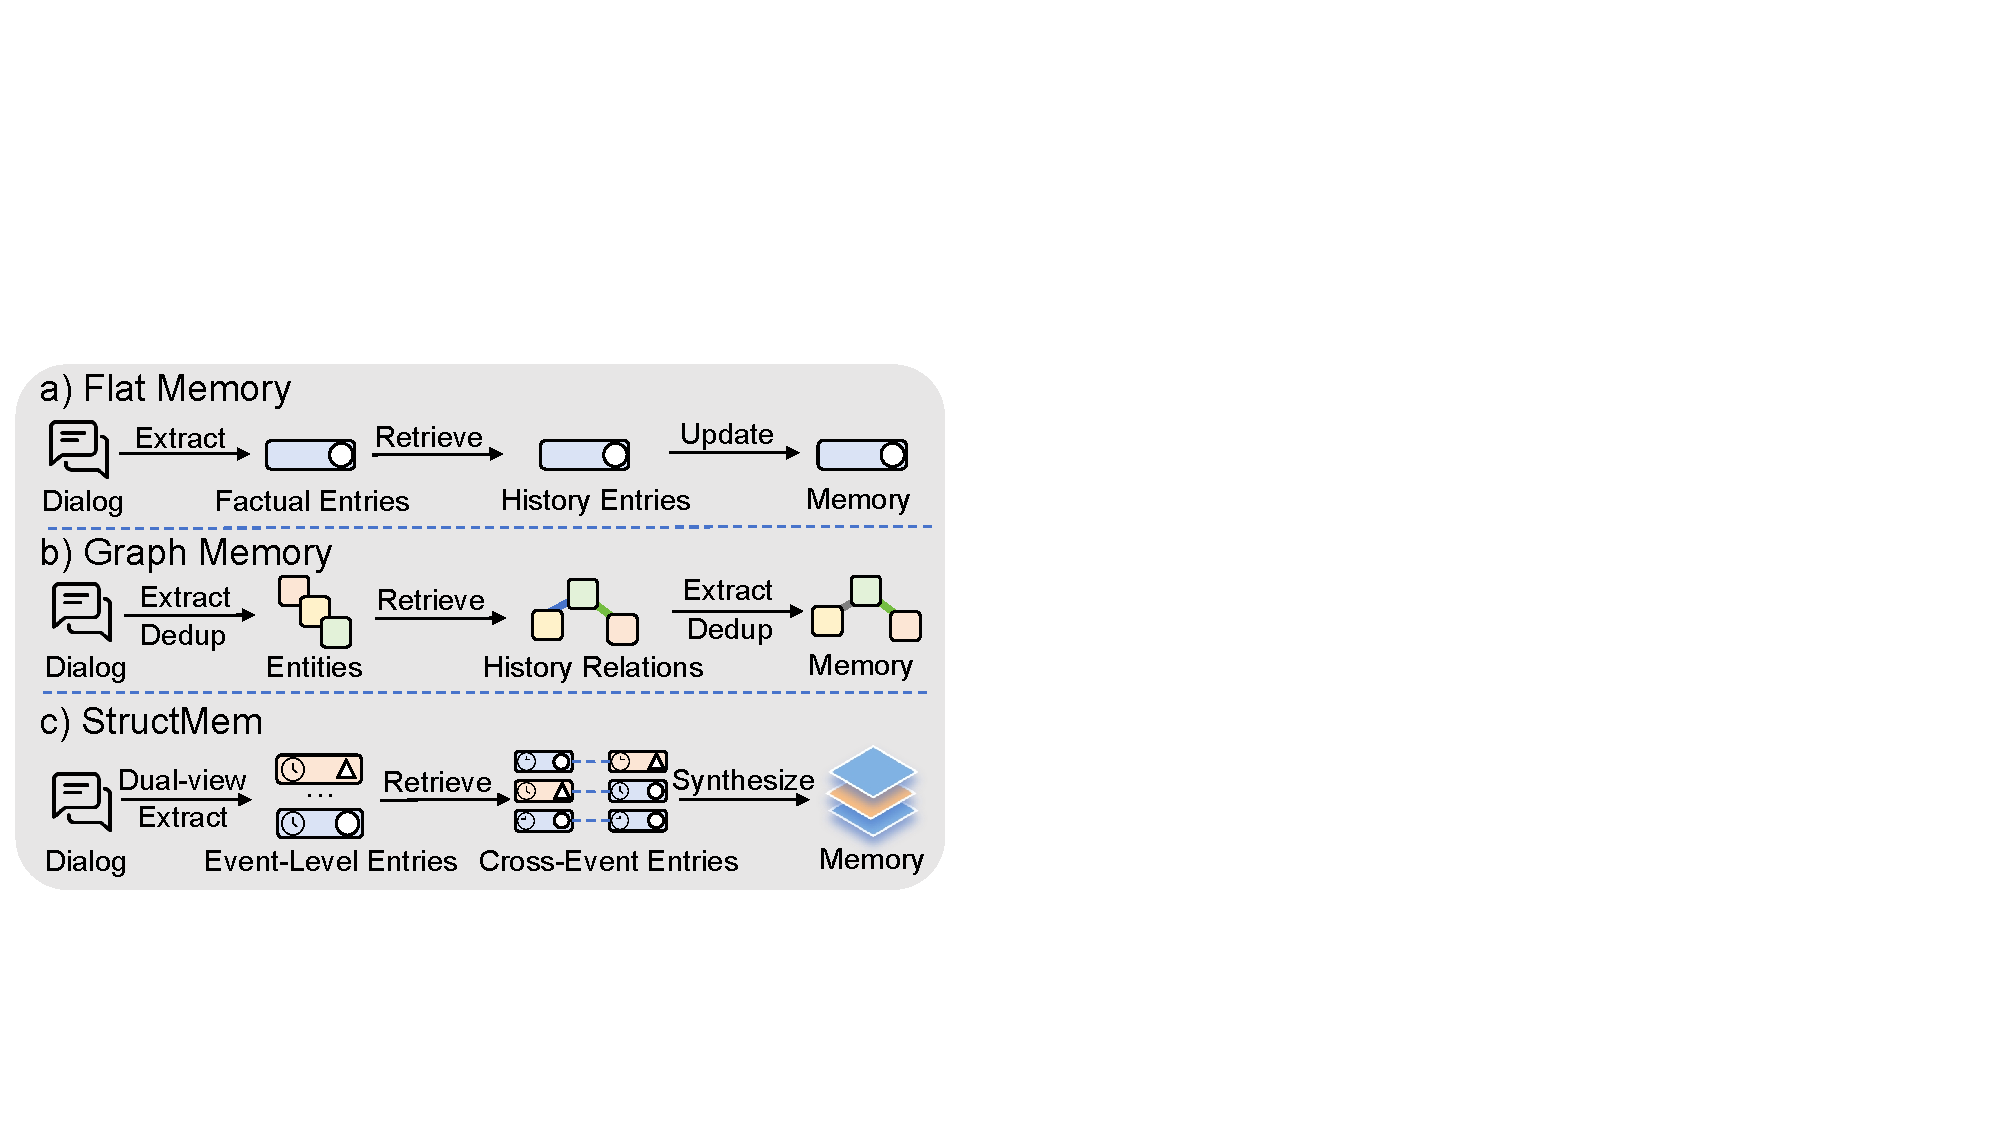
\includegraphics[width=0.99\linewidth]{figure/2026ACL-Intro.pdf}
    \caption{Three paradigms of Memory systems.}
    \vspace{-5mm}
    \label{fig:intro}
\end{figure}

 
Based on this insight, we propose \textbf{StructMem}, a hierarchical memory framework built around event-centric representations. This abstraction preserves both what happened and how events relate across agents and time, while avoiding explicit schema design, entity resolution, and symbolic graph traversal. 
Specifically, at the event level, StructMem constructs structured episodes through dual-perspective extraction, capturing both event content and interactional relations within temporal context. At the cross-event level, it performs periodic consolidation over semantically related events, exploiting temporal locality to efficiently induce higher-level relational structure. Experiments on \texttt{LoCoMo} show that StructMem improves long-horizon reasoning while significantly reducing computational overhead.
% To address these issues, we propose \textbf{StructMem}, a hierarchical framework built on a key insight: the fundamental unit of conversational memory should be temporally-grounded relational events, not isolated facts or entity-relation triplets. This abstraction preserves causal and interpersonal bindings within natural episodic context while avoiding rigid schemas and entity resolution overhead.

% \textbf{StructMem} realizes this through two complementary mechanisms. At the event level, dual-perspective extraction captures content memory representing event descriptions and interaction memory encoding relational dynamics, both anchored to temporal contexts. At the cross-event level, periodic synthesis consolidates semantically related events, exploiting temporal locality where related events naturally cluster to enable efficient batch consolidation. Experiments on \texttt{LoCoMo} show that \textbf{StructMem} achieves better performance while significantly reducing computational consumption.